% EXP instruction format

\documentclass[tikz,border=10pt]{standalone}
\begin{document}
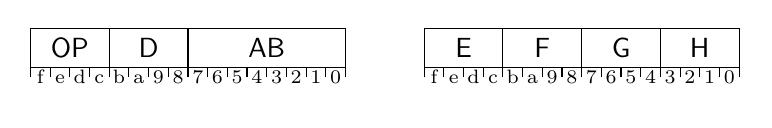
\begin{tikzpicture}

  \draw (0,0) rectangle (4,0.5);
  \draw (1,0) -- (1,0.5);
  \draw (2,0) -- (2,0.5);
  \foreach \x in {0, 0.25, ..., 4} \draw (\x,-0.1250) -- (\x,0);
  \foreach \i/\x in 
  {f/0.125, e/0.375, d/0.625, c/0.875,
    b/1.125, a/1.375, 9/1.625,
    8/1.875, 7/2.125, 6/2.375, 5/2.625,
    4/2.875, 3/3.125, 2/3.375, 1/3.625, 0/3.875}
  \draw (\x,-0.15) node {\scriptsize\textsf\strut\i};y 
  \draw (0.5,0.25) node {\textsf{OP}};
  \draw (1.5,0.25) node {\textsf{D}};
  \draw (3.0,0.25) node {\textsf{AB}};

  \begin{scope}[xshift=5cm]
    \draw (0,0) rectangle (4,0.5);
  \draw (1,0) -- (1,0.5);
  \draw (2,0) -- (2,0.5);
  \draw (3,0) -- (3,0.5);
    \foreach \x in {0, 0.25, ..., 4} \draw (\x,-0.1250) -- (\x,0);
    \foreach \i/\x in 
    {f/0.125, e/0.375, d/0.625, c/0.875,
      b/1.125, a/1.375, 9/1.625,
      8/1.875, 7/2.125, 6/2.375, 5/2.625,
      4/2.875, 3/3.125, 2/3.375, 1/3.625, 0/3.875}
    \draw (\x,-0.15) node {\scriptsize\textsf\strut\i};
  \draw (0.5,0.25) node {\textsf{E}};
  \draw (1.5,0.25) node {\textsf{F}};
  \draw (2.5,0.25) node {\textsf{G}};
  \draw (3.5,0.25) node {\textsf{H}};
  \end{scope}
  
\end{tikzpicture}
\end{document}

% Version with decimal indices 15, 14, ... (they are wide)
% \foreach \i/\x in 
%   {15/0.125, 14/0.375, 13/0.625, 12/0.875,
%    11/1.125, 10/1.375, 9/1.625,
%    8/1.875, 7/2.125, 6/2.375, 5/2.625,
%    4/2.875, 3/3.125, 2/3.375, 1/3.625, 0/3.875}
%  \draw (\x,-0.1250) node {\tiny$\i$};y

% Generate the coordinates with ghci; can't use ... notation
% when there are two simultaneous interator variables.

% ghci> [0.125, 0.375 .. 3.875]
% [0.125,0.375,0.625,0.875,1.125,1.375,1.625,
%  1.875,2.125,2.375,2.625,2.875,3.125,3.375,3.625,3.875]

% Here are the i/x pairs
%  [15/0.125, 14/0.375, 13/0.625, 12/0.875,
%  11/1.125, 10/1.375, 9/1.625,
%  8/1.875, 7/2.125, 6/2.375, 5/2.625,
%  4/2.875, 3/3.125, 2/3.375, 1/3.625, 0/3.875]
